\problem{Numerical Solutions by Euler's Approximation}

Implement and test Euler's approximation and compare iterative improvements to the true function.

\solution

\part 

First, Euler's approximation is tested by hand.
The function solves the initial value problem: 
$$y’ = f(t,y)$$
$$ y(t0) = y0$$ 
in the time interval $tspan = [t0,tf]$ using Euler’s method with $N$ time steps.

The code is condensed into the following form, as a function of: $f$, a mathematical function, $tspan$, an interval, $y0$, an initial value, and $N$, a number of intervals:

\begin{verbatim}
function [t, y] = euler(f, tspan, y0, N)
m = length(y0);
t0 = tspan(1);
tf = tspan(2);
h = (tf - t0)/N;
t = linspace(t0, tf, N+1);
y = zeros(m, N+1);
y(:,1) = y0';
for n = 1:N
    y(:,n+1) = y(:,n) + h*f(t(n), y(:,n));
end
t = t'; y = y';
end

\end{verbatim}

This code is then tested with the following function:

$$f(t, y) = 2y$$

For $N = 5, N = 50$, and the true solution, the following graph is created (next page).

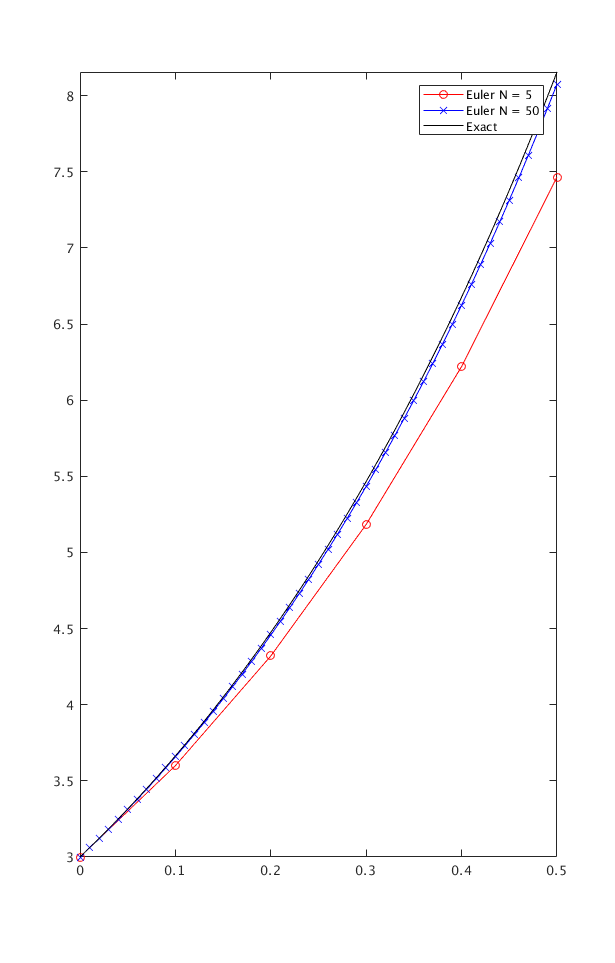
\includegraphics{approximation}

\part

The following exercises are solved:

\begin{enumerate}
    \item \emph{Create a table showing different approximations and their error:} \\ \\
        \begin{tabular}{l|l|l|l}
         N    & approximation & error & ratio \\
         \hline
         5    & 7.4650 & 0.6899 & 1 \\
         50   & 8.0748 & 0.0801 & 8.6148 \\
         500  & 8.1467 & 0.0082 & 84.7533 \\
         5000 & 8.1540 & 0.0008 & 846.1374
        \end{tabular}
    \item \emph{Examine the last column. How does the ratio of consecutive errors relate to the number of steps used? Your answer to this question should confirm the fact that Euler’s method is of “order h”, that is, every time the stepsize is decreased by a factor k, the error is also reduced (approximately) by the same factor.} \\ \\
        The error ratio is increasing linearly with the number of intervals, which confirms that Euler's method is $O(h)$. To confirm this, consider the formula $err_{ratio} = \frac{N}{5} * 8.461374$, which approximates the error ratio as a \emph{linear} function of number of intervals quite well.
    \item \emph{Recall the geometrical interpretation of Euler’s method based on the tangent line. Using this geometrical interpretation, can you explain why the Euler approximations underestimate the solution in this particular example?} \\ \\
        In this particular example, the true curve is $y^2$, hence the derivative is $f(t, y) = 2y$. From this, when a tangent line is drawn, it lies below the parabola, and does not curve upwards (by nature of being a line). This creates space between the tangent line and the true curve. Since a finite step is being taken along the tangent line, this space is unaccounted for, and error is created. In this case, the error is an underestimation because the parabola curves upwards and thus the tangent line is literally \emph{under} the curve for any positive $t$.  
\end{enumerate}
